\documentclass[journal, a4paper]{IEEEtran}

% Add the compsoc option for Computer Society conferences.
%
% If IEEEtran.cls has not been installed into the LaTeX system files,
% manually specify the path to it like:
% \documentclass[conference]{../sty/IEEEtran}

\usepackage{mathtools}
\usepackage{hyperref}
\usepackage{subfigure}
\usepackage[pdftex]{graphicx}
\graphicspath{{./fig/}}
\DeclareGraphicsExtensions{.pdf,.jpeg,.png}
\usepackage{todonotes}
\usepackage[nodayofweek]{datetime}

\newdateformat{dday}{
	\monthname[\THEMONTH], \THEYEAR
}


% Some very useful LaTeX packages include:
% (uncomment the ones you want to load)


% *** MISC UTILITY PACKAGES ***
%
%\usepackage{ifpdf}
% Heiko Oberdiek's ifpdf.sty is very useful if you need conditional
% compilation based on whether the output is pdf or dvi.
% usage:
% \ifpdf
%   % pdf code
% \else
%   % dvi code
% \fi
% The latest version of ifpdf.sty can be obtained from:
% http://www.ctan.org/tex-archive/macros/latex/contrib/oberdiek/
% Also, note that IEEEtran.cls V1.7 and later provides a builtin
% \ifCLASSINFOpdf conditional that works the same way.
% When switching from latex to pdflatex and vice-versa, the compiler may
% have to be run twice to clear warning/error messages.






% *** CITATION PACKAGES ***
%
%\usepackage{cite}
% cite.sty was written by Donald Arseneau
% V1.6 and later of IEEEtran pre-defines the format of the cite.sty package
% \cite{} output to follow that of IEEE. Loading the cite package will
% result in citation numbers being automatically sorted and properly
% "compressed/ranged". e.g., [1], [9], [2], [7], [5], [6] without using
% cite.sty will become [1], [2], [5]--[7], [9] using cite.sty. cite.sty's
% \cite will automatically add leading space, if needed. Use cite.sty's
% noadjust option (cite.sty V3.8 and later) if you want to turn this off.
% cite.sty is already installed on most LaTeX systems. Be sure and use
% version 4.0 (2003-05-27) and later if using hyperref.sty. cite.sty does
% not currently provide for hyperlinked citations.
% The latest version can be obtained at:
% http://www.ctan.org/tex-archive/macros/latex/contrib/cite/
% The documentation is contained in the cite.sty file itself.






% *** GRAPHICS RELATED PACKAGES ***
%


  % or other class option (dvipsone, dvipdf, if not using dvips). graphicx
  % will default to the driver specified in the system graphics.cfg if no
  % driver is specified.
  % \usepackage[dvips]{graphicx}
  % declare the path(s) where your graphic files are
  % \graphicspath{{../eps/}}
  % and their extensions so you won't have to specify these with
  % every instance of \includegraphics
  % \DeclareGraphicsExtensions{.eps}

% graphicx was written by David Carlisle and Sebastian Rahtz. It is
% required if you want graphics, photos, etc. graphicx.sty is already
% installed on most LaTeX systems. The latest version and documentation can
% be obtained at: 
% http://www.ctan.org/tex-archive/macros/latex/required/graphics/
% Another good source of documentation is "Using Imported Graphics in
% LaTeX2e" by Keith Reckdahl which can be found as epslatex.ps or
% epslatex.pdf at: http://www.ctan.org/tex-archive/info/
%
% latex, and pdflatex in dvi mode, support graphics in encapsulated
% postscript (.eps) format. pdflatex in pdf mode supports graphics
% in .pdf, .jpeg, .png and .mps (metapost) formats. Users should ensure
% that all non-photo figures use a vector format (.eps, .pdf, .mps) and
% not a bitmapped formats (.jpeg, .png). IEEE frowns on bitmapped formats
% which can result in "jaggedy"/blurry rendering of lines and letters as
% well as large increases in file sizes.
%
% You can find documentation about the pdfTeX application at:
% http://www.tug.org/applications/pdftex





% *** MATH PACKAGES ***
%
%\usepackage[cmex10]{amsmath}
% A popular package from the American Mathematical Society that provides
% many useful and powerful commands for dealing with mathematics. If using
% it, be sure to load this package with the cmex10 option to ensure that
% only type 1 fonts will utilized at all point sizes. Without this option,
% it is possible that some math symbols, particularly those within
% footnotes, will be rendered in bitmap form which will result in a
% document that can not be IEEE Xplore compliant!
%
% Also, note that the amsmath package sets \interdisplaylinepenalty to 10000
% thus preventing page breaks from occurring within multiline equations. Use:
%\interdisplaylinepenalty=2500
% after loading amsmath to restore such page breaks as IEEEtran.cls normally
% does. amsmath.sty is already installed on most LaTeX systems. The latest
% version and documentation can be obtained at:
% http://www.ctan.org/tex-archive/macros/latex/required/amslatex/math/





% *** SPECIALIZED LIST PACKAGES ***
%
%\usepackage{algorithmic}
% algorithmic.sty was written by Peter Williams and Rogerio Brito.
% This package provides an algorithmic environment fo describing algorithms.
% You can use the algorithmic environment in-text or within a figure
% environment to provide for a floating algorithm. Do NOT use the algorithm
% floating environment provided by algorithm.sty (by the same authors) or
% algorithm2e.sty (by Christophe Fiorio) as IEEE does not use dedicated
% algorithm float types and packages that provide these will not provide
% correct IEEE style captions. The latest version and documentation of
% algorithmic.sty can be obtained at:
% http://www.ctan.org/tex-archive/macros/latex/contrib/algorithms/
% There is also a support site at:
% http://algorithms.berlios.de/index.html
% Also of interest may be the (relatively newer and more customizable)
% algorithmicx.sty package by Szasz Janos:
% http://www.ctan.org/tex-archive/macros/latex/contrib/algorithmicx/




% *** ALIGNMENT PACKAGES ***
%
%\usepackage{array}
% Frank Mittelbach's and David Carlisle's array.sty patches and improves
% the standard LaTeX2e array and tabular environments to provide better
% appearance and additional user controls. As the default LaTeX2e table
% generation code is lacking to the point of almost being broken with
% respect to the quality of the end results, all users are strongly
% advised to use an enhanced (at the very least that provided by array.sty)
% set of table tools. array.sty is already installed on most systems. The
% latest version and documentation can be obtained at:
% http://www.ctan.org/tex-archive/macros/latex/required/tools/


%\usepackage{mdwmath}
%\usepackage{mdwtab}
% Also highly recommended is Mark Wooding's extremely powerful MDW tools,
% especially mdwmath.sty and mdwtab.sty which are used to format equations
% and tables, respectively. The MDWtools set is already installed on most
% LaTeX systems. The lastest version and documentation is available at:
% http://www.ctan.org/tex-archive/macros/latex/contrib/mdwtools/


% IEEEtran contains the IEEEeqnarray family of commands that can be used to
% generate multiline equations as well as matrices, tables, etc., of high
% quality.


%\usepackage{eqparbox}
% Also of notable interest is Scott Pakin's eqparbox package for creating
% (automatically sized) equal width boxes - aka "natural width parboxes".
% Available at:
% http://www.ctan.org/tex-archive/macros/latex/contrib/eqparbox/





% *** SUBFIGURE PACKAGES ***
%\usepackage[tight,footnotesize]{subfigure}
% subfigure.sty was written by Steven Douglas Cochran. This package makes it
% easy to put subfigures in your figures. e.g., "Figure 1a and 1b". For IEEE
% work, it is a good idea to load it with the tight package option to reduce
% the amount of white space around the subfigures. subfigure.sty is already
% installed on most LaTeX systems. The latest version and documentation can
% be obtained at:
% http://www.ctan.org/tex-archive/obsolete/macros/latex/contrib/subfigure/
% subfigure.sty has been superceeded by subfig.sty.



%\usepackage[caption=false]{caption}
%\usepackage[font=footnotesize]{subfig}
% subfig.sty, also written by Steven Douglas Cochran, is the modern
% replacement for subfigure.sty. However, subfig.sty requires and
% automatically loads Axel Sommerfeldt's caption.sty which will override
% IEEEtran.cls handling of captions and this will result in nonIEEE style
% figure/table captions. To prevent this problem, be sure and preload
% caption.sty with its "caption=false" package option. This is will preserve
% IEEEtran.cls handing of captions. Version 1.3 (2005/06/28) and later 
% (recommended due to many improvements over 1.2) of subfig.sty supports
% the caption=false option directly:
%\usepackage[caption=false,font=footnotesize]{subfig}
%
% The latest version and documentation can be obtained at:
% http://www.ctan.org/tex-archive/macros/latex/contrib/subfig/
% The latest version and documentation of caption.sty can be obtained at:
% http://www.ctan.org/tex-archive/macros/latex/contrib/caption/




% *** FLOAT PACKAGES ***
%
%\usepackage{fixltx2e}
% fixltx2e, the successor to the earlier fix2col.sty, was written by
% Frank Mittelbach and David Carlisle. This package corrects a few problems
% in the LaTeX2e kernel, the most notable of which is that in current
% LaTeX2e releases, the ordering of single and double column floats is not
% guaranteed to be preserved. Thus, an unpatched LaTeX2e can allow a
% single column figure to be placed prior to an earlier double column
% figure. The latest version and documentation can be found at:
% http://www.ctan.org/tex-archive/macros/latex/base/



%\usepackage{stfloats}
% stfloats.sty was written by Sigitas Tolusis. This package gives LaTeX2e
% the ability to do double column floats at the bottom of the page as well
% as the top. (e.g., "\begin{figure*}[!b]" is not normally possible in
% LaTeX2e). It also provides a command:
%\fnbelowfloat
% to enable the placement of footnotes below bottom floats (the standard
% LaTeX2e kernel puts them above bottom floats). This is an invasive package
% which rewrites many portions of the LaTeX2e float routines. It may not work
% with other packages that modify the LaTeX2e float routines. The latest
% version and documentation can be obtained at:
% http://www.ctan.org/tex-archive/macros/latex/contrib/sttools/
% Documentation is contained in the stfloats.sty comments as well as in the
% presfull.pdf file. Do not use the stfloats baselinefloat ability as IEEE
% does not allow \baselineskip to stretch. Authors submitting work to the
% IEEE should note that IEEE rarely uses double column equations and
% that authors should try to avoid such use. Do not be tempted to use the
% cuted.sty or midfloat.sty packages (also by Sigitas Tolusis) as IEEE does
% not format its papers in such ways.





% *** PDF, URL AND HYPERLINK PACKAGES ***
%
%\usepackage{url}
% url.sty was written by Donald Arseneau. It provides better support for
% handling and breaking URLs. url.sty is already installed on most LaTeX
% systems. The latest version can be obtained at:
% http://www.ctan.org/tex-archive/macros/latex/contrib/misc/
% Read the url.sty source comments for usage information. Basically,
% \url{my_url_here}.




\newcommand{\reffig}[1]{Fig. \ref{#1}}

\hyphenation{op-tical net-works semi-conduc-tor}


\begin{document}

\title{Survey paper of techniques for optimizing DRAM refresh}

\author{\IEEEauthorblockN{Dan Larsson, Jonas Hemlin}\\
\IEEEauthorblockA{Master Program of Embedded Electronic Systems Design\\
Chalmers University of Technology, Gothenburg, Sweden\\
Email: \{larsdan, jhemlin\}@student.chalmers.se}}

\maketitle


\begin{abstract}
We survey nine different techniques for lowering the number of refresh operations performed in a modern DRAM system. Because the portion of power consumption coming from refresh operations in DRAM is high and increasing, these techniques are both topical and highly considerable. The relative performance of the techniques is compared, and some projections for the future concerning higher density and bigger capacity DRAMs are discussed. The new ways to improve DRAM, like 3D stacked DRAM, will increase the need to mitigate refresh power even further. To give a context to the techniques surveyed the basic operation of DRAM is elaborated on. 

All the techniques surveyed fits into one or more approach, where each approach utilizes on of four types of information, Retention Time, Access Recency, Data Tolerance, or Validity. Among these approaches, we believe that Retention Time and Validity are the most promising as their benefits manage to scale well with DRAM capacity. Moreover, they show large improvements to a relatively low complexity, compared to the others.
\end{abstract}

\section{Introduction}
\label{sec:int}
These laboratory assignments aim to increase our knowledge of different cache coherence protocols. To reach this goal, we simulate cache coherence protocols (CCP) on a modeled cache coherent multi-core system using diverse benchmarks. Three cache coherence protocols are targeted; MSI, MESI, and MESI-MG, where the last protocol is an modified version of MESI optimized for migratory sharing. The system model have a shared Last Level Cache (LLC), and each processor have a private L1 cache. Snooping based write-invalidate cache coherence protocols are used by the private L1 caches to ensure coherence, and a simple bus stand for the communication between LLC and private caches. The system is modeled by the Pin tool MultiCacheSim and Pin. In listing~\ref{lst:setup} is the command used for simulating a CCP on the modeled system with a chosen benchmark. To relate the simulation results to excecution time, Eq. \ref{eq:cycles} is used. 



\begin{lstlisting}[label=lst:setup, basicstyle=\scriptsize, caption={Command used for simulation.}]
#> ./pin -mt -t ./source/tools/MultiCacheSim/obj-intel64/mcs.so -csize 65536 -bsize 64 -assoc 8 -llc -llcsize 4194304 -llcbsize 64 -llcassoc 16 -numcaches 8 -protos ./source/tools/MultiCacheSim/obj-intel64/mcs_<CCP>.so -- <benchmark> [#threads,..]
\end{lstlisting}
\begin{equation}
	$$\label{eq:cycles}$$
	Cycles = 1 * (WriteHit+ReadHit) + 30 * (readMissesServicedByModified + invalidationsSent)$$ $$+ 20 * LLCHit + 50 * LLCMiss
\end{equation}
\section{Background} 
\label{sec:bg}
In this section we give a brief overview of DRAM, covering the organization, basic operation, refresh modes, and trends together with projections for the DRAM structure.

DRAM is hierarchically organized as in \reffig{fig:dram_orga}. At the top of the hierarchy are the \textit{channels} that are connected to one or more \textit{ranks}, each composed of multiple storage arrays called \textit{banks}. Each channel has individual address, data, and command buses that makes it possible for the channels to operate concurrently. All ranks on one channel can operate in parallel, but are constrained by the channel bandwidth, which is shared among the ranks. Further, the banks within the ranks operate in parallel, but are constrained by both the shared channel bandwidth and resources shared among the banks. 

The DRAM cell array in each bank is structured as in \reffig{fig:dram_orgb}. One cell consists of a transistor and a capacitor, where the transistor is controlled by the \textit{word line} wire and connects the capacitor to the \textit{bit line} wire. The word line connects a number of cells which forms a row. Each bit line is connected to a sense amplifier, and the row of sense amplifiers constitutes the \textit{row buffer}. Data is stored as a charge on the cell capacitor.

\begin{figure*}[t]
    \centering
    \subfigure[DRAM hierarchy]{
        \centering
        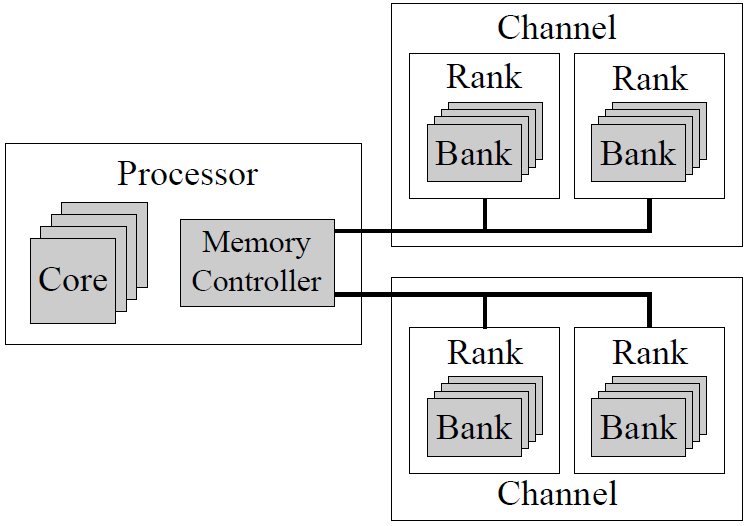
\includegraphics[width=0.4\textwidth]{dram_orga}
		\label{fig:dram_orga}
    }
    \subfigure[DRAM bank structure]{
        \centering
        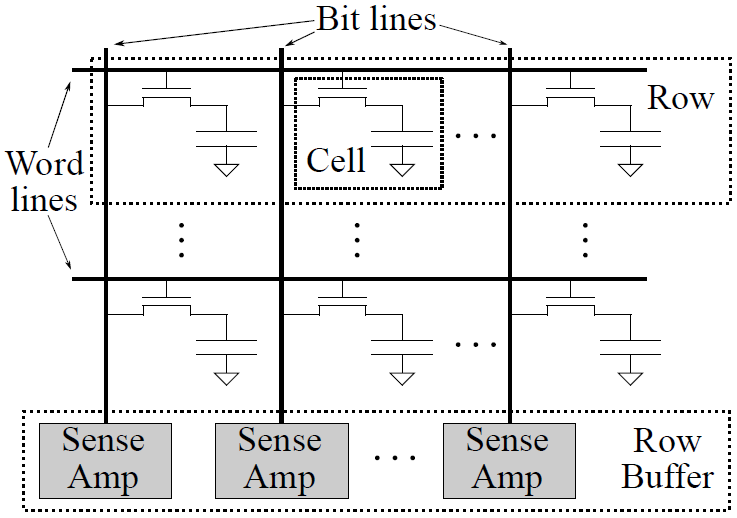
\includegraphics[width=0.4\textwidth]{dram_orgb}
		\label{fig:dram_orgb}
    }
	\caption{DRAM system organization \cite{raidr}.}
	\label{fig:dram_org}
\end{figure*}

To read a row, the word line connected to the row's transistors must first be activated. When the word line is activated, the transistors connect the capacitors to the bit lines. When the capacitors connect to the bit lines, charge will either flow from or to the capacitors depending on whether they were charged or not, respectively. For this to work, the bit lines have to be precharged to $V_{DD}/2$. The sense amplifiers then detect the change of voltage, which makes it possible to interpret the stored data. The charge stored on the capacitors has, as mentioned, left the capacitor and a read operation is thus destructive. To maintain the data the capacitors are recharged by the bit lines, which are driven to either either $V_{DD}/2$ or $0\:V$ by the sense amplifiers depending on the former voltage detected. Finally, when another row on the bank is accessed, the open row has to be closed, which disconnects the capacitors from the bit lines.

To write to a row, the corresponding word line is first activated. As during a read, the transistors then connect the capacitors to the bit lines, and charge will either flow from or to the capacitor. The row buffer is then loaded with the data that are driven to the bit lines by the sense amplifiers, thus storing the information on the capacitors. The row will be closed when another row is accessed.

As mentioned, the capacitors leak charge over time and have to be recharged in order to preserve the data. The refresh is performed by opening a row to let the sense amplifiers magnify the detected voltage change and thus recharge the cells to either $V_{DD}/2$ or $0\:V$. This follows the same procedure as a read operation and thus is the row always refreshed when a read is performed. % Is it clear that the row is refreshed during a write?

The memory controller (MC) normally issues refresh operations periodically at an interval of $64\:ms$ for each row, an interval that has been constant for the latest DRAM specifications [source] and called \textit{maximum refresh period}. This interval is conservatively halved if the DRAM exceeds the specified working temperature of $85^{\circ}C$. 

To refresh one rank, the simplest approach is to refresh all banks in parallel row-by-row at the start of the $64\:ms$ interval. This approach is called \textit{burst refresh}. The approach blocks normal accesses for a long period, and power consumption peaks during the burst time. A better alternative is to use \textit{distributed refresh}, which scatter the refreshes across the interval, resulting in a lower average latency for the processor and more stable power consumption.

The implementation of a DRAM refresh cycle can be made in two different ways, to either affect one row or many. The first is called \textit{RAS-only refresh} (ROR) where a refresh cycle refreshes one targeted row. To target one row, the row's address is put on the bus, and the MC have the responsibility that a row is refreshed within the maximum refresh period. The second is called \textit{CAS before RAS refresh} (CBR). In this scheme, the memory module have an internal address counter that displays which row that will be refreshed. On a refresh cycle, the row stated by the internal address counter is refreshed and the counter is then incremented. Contrary to ROR, CBR do not need provided addresses on the bus, which results in a lower power consumption and less bus usage. % During CBR, a row in each bank is updated, right? if so. write that in the text.

When using CBR, all banks in a rank are blocked for normal accesses. All banks are also blocked when ROR is used due to DRAM chip design, however some DRAM chips support per-bank refresh commands that makes it possible to only block the specific bank being refreshed. 

\begin{figure}[t]
    \centering
    \subfigure[DRAM throughput loss]{
        \centering
        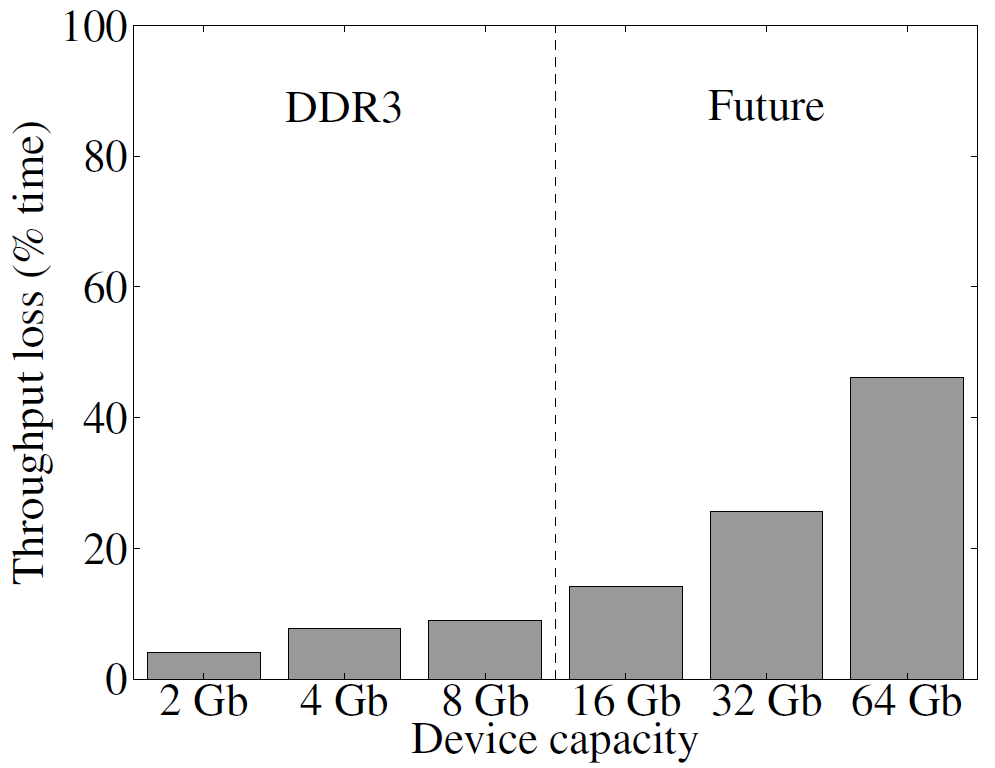
\includegraphics[width=0.33\textwidth]{dram_throughput}
        \label{fig:dram_throughput}
    }
    \subfigure[DRAM power consumption]{
        \centering
        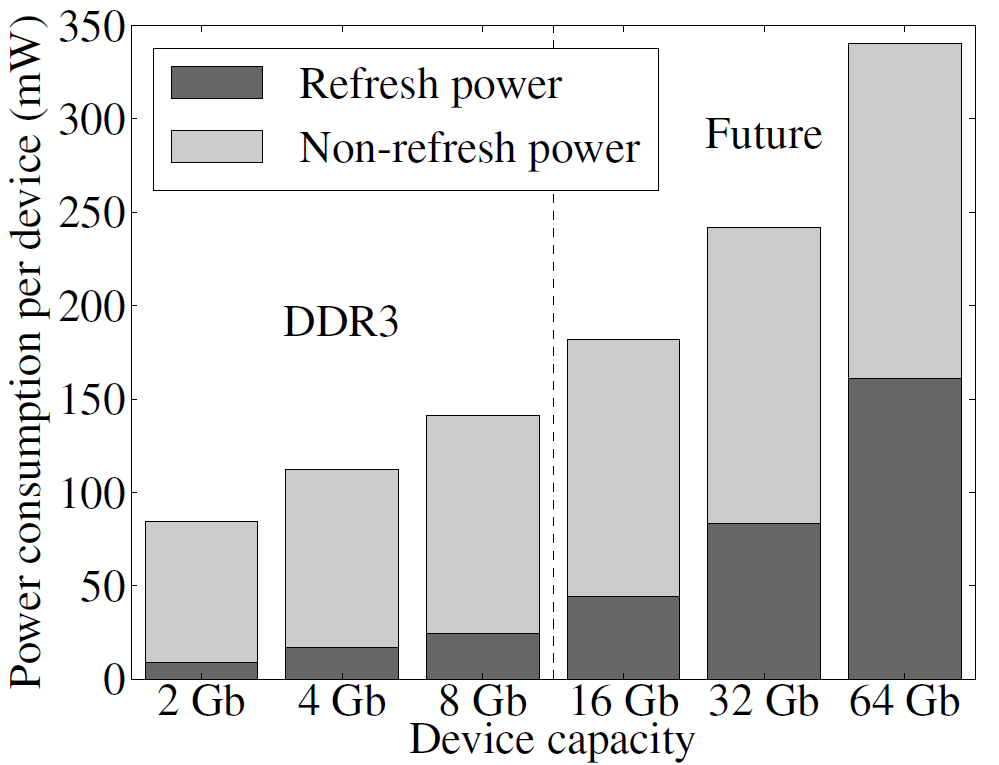
\includegraphics[width=0.33\textwidth]{dram_power}
        \label{fig:dram_power}
    }
    \caption{Projections on DRAM throughput loss and power consumption in extended-temperature operation \cite{raidr}.}
    \label{fig:dram_data_proj}
\end{figure}

The trends in DRAM chips is to increase capacity with each generation. In practice, this is realized to a high degree by adding additional rows in the banks. The rows could instead - or also - been made longer by adding DRAM cells, but this solution is not favorable as it increases the power consumption per row access. 

As refresh operations are made by row, the refresh operations will increase linearly with the device capacity. In turn, the throughput loss increases exponentially, as shown in \reffig{fig:dram_throughput}. Additional refresh operations give larger power consumption and the refreshes become a growing portion of the total DRAM energy consumption, as shown in \reffig{fig:dram_power}. When the device capacity reaches $64\:GB$, the refresh power nearly constitutes half of the total consumption, an increase from 15\% if the device capacity is 8 GB. 

The conclusion to draw from \reffig{fig:dram_data_proj} is that it will be increasingly important to mitigate the throughput loss and DRAM power consumption of future systems. One way to decrease these negative trends of DRAM scaling is to optimize the DRAM refresh. However, a reduction in the number of refreshes made has no linear relationship to the reduction in refresh energy consumption. The energy reduction depends on the state of the bank in which the targeted row resides; if the targeted row is closed more energy will be consumed than if the targeted row would have been open.
\section{Reducing refresh power} 
\label{sec:red}
There are several approaches to decrease the refresh power by reducing unnecessary refreshes and these can be categorized depending on which sort of information the scheduling decisions are based upon. The four types of information are: access recency, cell retention time, error tolerance of the data, and line validity. This categorization follows the taxonomy proposed by Cui et al. \cite{dtail}. These four approaches are explained further in \ref{sec:red:app}, whereas techniques based on the approaches are summarized in \ref{sec:red:tech}. 

\subsection{Approaches to reduce refresh power}
\label{sec:red:app}

\subsubsection*{\textbf{Access Recency (A)}}
As mentioned, a DRAM access is performed in the same way as a refresh, which makes it possible to delay the next refresh operation to an accessed row without endangering the stored data. All accessed rows within the maximum refresh period result in that a refresh can be postponed. This implies that if the system seldom accesses the DRAM data, or only a small portion of it, the approach's gain diminishes.


\subsubsection*{\textbf{Retention Time (R)}}
The need for refresh is as mentioned caused by leakage in the memory cells. Retention time is a measurement of the time it takes before a cell loose its data if not refreshed (recharged). Variations in the manufacturing process causes a exponentially distributed fluctuation \cite{katayama} in the retention time of the DRAM cells. To accommodate for the cells with the lowest retention time, manufacturers produce chips with average retention times much higher than possible minimum. This gives room for optimization using variable refresh rate for different cells. The retention time is also highly sensitive to temperature variations and becomes drastically lower at higher temperatures. For techniques using this approach the biggest advantage is that the improvements are independent of workload, except for a potential rise in temperature which would lower the retention time.

\subsubsection*{\textbf{Data Tolerance (T)}}
In the other approaches all data loss is seen as intolerable. In this approach data is categorized depending on how critical it is, which yields that cells containing data with a lower criticality may be refreshed more seldom. Applications such as approximate computations, games, or media processing can tolerate some bit errors while still producing a acceptable result. Using this approach, the energy and performance savings achieved is highly depending on what kind of applications most commonly are run on the system. 

\subsubsection*{\textbf{Validity (V)}}
In a system that does not utilize all the available memory space it is unnecessary to refresh parts not used. Therefore, cells that do not keep valid data do not need to be refreshed. The allocation and deallocation of the cells have to be tracked to get the information needed for implementation. This approach is highly sensitive to memory utilization of the system and its effects on energy consumption and performance improvements will be diminishing on systems with high workload.  

\subsection{Techniques to reducing refresh power}
\label{sec:red:tech}

\subsubsection*{\textbf{Smart Refresh}}
\label{par:smartrefresh}
The basic concept behind our scheme is that a memory line that has been recently read out or written to does not need to be refreshed again by the periodic refresh mechanism.

Uses a time-out counter for each memory line. The counter is set on a read/write/refresh and dicards refreshes until the timer hits zero. The counter is associated to a bank/line pair. The counters are stored in the memory controller. One counter consists of 2 SRAM bits. More bits give higher granularity and thus also better performance because the refresh is made less often.

This scheme will be most effective if all lines are accessed before a refresh is needed. If no accesses are made = the entire working set fits into cache, Smart Refresh becomes CBR (CAS before RAS). Only refresh one line at a time = inefficient, so they have made it possible to turn the technique off.

Implemented so only one line per each logical segments are deremented at the same time, which leads to that the refreshes are evenly distributed over time. (I.e. no burst refresh.)

Overhead: 48KB for 2GB and 768 KB for 32GB = 0,0024\% overhead. 

Average reduction of refreshes by 59.3\% for 2GB and 52.3\% energy saving regarding the DRAM refresh. No performance degradation.

Employed its solution to 2 GB ram. What about todays sizes? How effective is the technique now? - Only works effective if large parts the memory is acccessed, i.e. large part of the memory has to be valid to begin with. Is it so today?

\subsubsection*{\textbf{Refrint}}
\label{par:refrint}
This technique is proposed by Agrawal et al. \cite{refrint} and is based on Access Recency. It is targeted towards caches and eDRAM, and thus can not be directly compared with the other solutions, but the main concept is of good use and the technique could be implemented DRAM as well. The concept is based on two types of unnecessary refreshes which originate from so called cold and hot rows. Cold rows are those used far apart in time or not used at all. The technique identifies and refreshes only those rows which are expected to be accessed in the near future, the rows that are used less frequent is invalidated. Hot rows consist of the rows that gets accessed frequently and thus can the technique postpone the preceding refresh to the accessed rows.

For the hot rows, an approach similar to Smart Refresh is employed. The differences are that Refrint does not maintain a counter for each row, but a snapshot of a global counter as well as the row's valid bit. When a row is accessed, the corresponding snapshot is updated with the current value of the global counter. Whenever the global counter steps to a new value, all normal accesses are stalled and the logic checks whether any of the valid row's snapshot  matches the global counter. If there is a match, a refresh is scheduled or the row is invalidated depending on the polices used for the cold rows. 

Four different policies can be applied for the cold rows, where the policies decide what to refresh; \textit{All}, \textit{Valid}, \textit{Dirty}, or \textit{WB(n,m)}. \textit{All} refreshes every row, regardless of whether it is valid or not. \textit{Valid} and \textit{Dirty} refreshes valid and dirty rows, respectively, and otherwise invalidate the row. \textit{WB(n,m)} refreshes a dirty row $n$ times before flushing it and changing the row state to valid clean, then the row is refreshed $m$ times after the last access before it is invalidated. $n$ and $m$ are time-out counters that are decremented upon refresh.

\todo[inline]{Drafty text below!}

Depending on the application's memory footprint and cache visibility the program is categorized to maximize the gain of the policies for cold rows. Visibility correspond to the amount of cache row accesses made by the application. If the application has high visibility, \textit{WB} is used and if the visibility is low, \textit{Valid} is used. A high visibility and a small footprint works best with small $n$ and $m$, whereas a large footprint is likely more usefull with small \textit{n} and \textit{m}. 

The technique modifies the MC. Which modifications and how large overhead? 5 bit snapshot for each row + state and n+m counters. some logic as well.

Presents the results. Add that we can not really use the result as they are from eDRAM.


\subsubsection*{\textbf{RAIDR}}
\label{par:raidr}
In this approach, RAIDR by Liu et al. \cite{raidr}, all memory rows get divided into different groups, called bins, based on the cell with the shortest Retention Time in the row. In the basic configuration there are two bins, one with rows that need a refresh rate of $64\:ms \to 128\:ms$ and one with rows that need to be refreshed every $128\:ms \to 256\:ms$. Rows in the first bin gets refreshed every $64\:ms$, rows in the second bin every $128\:ms$, and all remaining rows gets refreshed at the default refresh rate which is set to $256\:ms$. This is done using two counters, one address counter that rolls over every $64\:ms$, and one counter that keeps track on how many times the address counter have rolled over. With this, every row will get selected as refresh candidate every $64\:ms$ and the refresh will be performed depending on which bin the row belongs to and on the second counter's value. The actual refreshes are performed by activating the row in question, essentially performing a ROR. RAIDR conform to temperature variations by utilizing a third counter that is used to scale all bins refresh rate with the temperature.

The technique is realized by modifying the MC. To minimize the storage needed for keeping track of bin members, Bloom filters are used. Thanks to this, only \textit{1.25 KB} storage is needed for a \textit{32 GB} (\textit{8 KB} row size) DRAM with the default configuration, which becomes \textit{0.031\%}. The storage requirement increases together with the number of bins used, while the granularity, thereby the decrease in refresh operations, of the technique becomes higher with more bins. Similarly to the number of bins, the size chosen for the Bloom filters also affects the storage overhead. 

Liu et al. evaluates twelve different configurations ranging from one bin with small Bloom filters to three bins with large Bloom filters. The latter gives the highest decrease in refresh operations but needs \textit{65.25 KB} of memory, while the first only needs \textit{64 B} but have much smaller impact on the number of refreshes performed. The default configuration is a trade of between these two extremes, and with it, a performance improvement of $4.1\%$, a decrease in power consumption by $8.3\%$, and a total reduction of refresh operations by $74.6\%$, is achieved in a \textit{32 GB} system compared to CBR.

\subsubsection*{\textbf{DTail}}
\label{par:dtail}
Cui et al. \cite{dtail} propose DTail. They evaluate two versions of DTail referenced as DTail-R and DTail-V utilizing Retention Time and Validity information, respectively. Even so, their main idea is that more types of refresh information can be incorporated and stored together with the Retention time and Validity information. DTail can then choose the most efficient refresh schema depending on the current situation, i.e. workload and type of application. Refresh data is kept per row and is stored in the DRAM itself instead of storing it in the MC which many other solutions do \cite{raidr}\cite{smartrefresh}\cite{refrint}. To counter the added latency of a slower memory, Cui et al. utilizes spatial locality of the refresh data and performs prefetching into a FIFO buffer. As the refresh data is kept on a row level DTail can save more refreshes than other techniques that have a lower granularity.

For DTail-R, the Retention Time data $n$ consists of three bits and is interpreted in such way that the refresh period can become \(64\:ms \times 2^n, n = [0..7]\). With DTail-V, one additional bit is added to the refresh data which is used to indicate if the row is valid or not. With this structure of four bits per row, the amount of memory required is $0.006\%$ of DRAM capacity assuming a row size of \textit{8 KB}.

When a row is selected for refresh by the memory controller, DTail intercepts the refresh command and based on the Retention Time and Validity information either lets the refresh to be performed or cancels it. The command used for refreshing a row depends on what is the most efficient at the time, if a large number of rows need refresh then CBR is selected, otherwise ROR is used. 

When only DTail-R is used, Cui et al. manages to decrease the number of refreshes with as much as $87.9\%$ and thereby only have $16.7\%$ energy overhead compared to a refresh less 32GB DRAM. With only DTail-V power consumption and performance overhead increase from $4\%$ and $3\%$ to $90\%$ and $23\%$, respectively, when going from $10\%$ to $90\%$ memory utilization compared to a refresh less 32 GB system. The power of DTail shows when DTail-R and DTail-V are used together and at $10\%$ memory utilization, a performance overhead of only $1\%$ and close to $0\%$ increase in energy consumption is achieved. When the utilization is increased to $90\%$, they increase to $2\%$ and $15\%$, respectively.

Comparing DTail with the somewhat similar RAIDR, Cui et al. achieves a bigger decrease in refresh operations compared to what Liu et al. does. This is due to DTail-R having a higher granularity as the refresh rate is kept per row and not per row group as in RAIDR.

\subsubsection*{\textbf{RIO and PARIS}}
\label{par:rioparis}
RIO is a technique proposed by S. Baek et al. \cite{rioparis} in which they identify cells with low retention time (bad cells) and `deletes' them. This is done by changing the memory allocating modules in the OS to not allocate pages that have bad cells in them. They implement RIO in a Linux kernel which is run and tested on a real hardware system and is able to achieve 87.5\% reduction in refresh count with a performance increas of 4.5\% on average. It is shown that going for a refresh period longer than \(256ms\) only yields a small performance and power improvment and therefore they does not try to push it higher. Their implementaion almost only relies on changes in the kernel and there is no need to modify the hardware so this technique would be easy to adopt in systems today. To keep fragmentation of the memory low a maximum of 0.1\% of total memory pages gets `deleted'. Even though deletion of a larger amount of pages could decrease the amount of refreshes further it would cause trouble for the kernel which relies on being able to allocate large contiguous address spaces. As retentiontime varies hugely with temperature RIO continously measures the system temperature and compensate the refresh persiod for it. S. Baek et al. also propose PARIS which can be combined with RIO for further improvments. In PARIS the goal is not to make the refresh period as long as possible but to not refresh unused memory cells at all. This is done by keeping track of memory pages allocated by the linux kernel.\todo[inline]{Write more about paris}

\subsubsection*{\textbf{SECRET}}
\label{par:secret}
With SECRET Lin et al. \cite{secret} masks cells with short retention time (bad cells) using Error Correction Pointers (ECP). The bad cells are mapped with a one time profiling done before first system use and all cells that do not meet the retention time requirements gets a ECP. A ECP is basically a pointer to another cell that is healthy. The framework, which is implemented inside the memory controller, checks whether there is any valid ECP for the address is accessed. If there is, it replaces the cell's data with the data from the cell pointed to by the ECP. The ECPs are stored in the DRAM during runtime and a cache in the memory controller is used to mask the delay of fetching the ECPs from DRAM.

The framework divides the DRAM into regions of typically \textit{128 KB}. For every one of these regions a \textit{Directory Entry} is kept. These directories holds the number of bad cells in the region and a address to where the ECPs are stored. As the Directory Entries need to be stored in a contiguous address space and the probability of that existing without any bad cell three copies are stored. A majority vote is then performed to mask any bit error in the Directory Entry. The size of each entry is $36\:b$ and all entries in a \textit{4 GB} system thus generates a total of $3 \times 36\:b \times \frac{4\:GB}{128\:KB} =$ \textit{432 KB} $= 0.010\%$ storage overhead. This is without the space needed for the actual ECPs which requires $21\:b$ each and the total space thereby varies with the number of bad cells.      

This approach gives a high energy saving of up to $87.2\%$ in refresh power and a reduction of $18.57\%$ in total DRAM power consumption with the ECP cache overhead taken into account and the refresh rate set to $512\:ms$ instead of the default $64\:ms$. The performance impact ranges from $1.3\%$ degradation at the worst to a $1.4\%$ improvement at the best. The degradation of performance is due to the added memory access needed to fetch the ECPs, and the performance improvement comes from the decreased congestion due to less refresh operations performed.

\subsubsection*{\textbf{Flikker}}
\label{par:flikker}
%flikker
Tolerance!

\subsubsection*{\textbf{Sparkk}}
\label{par:sparkk}
%Sparkk
Lucas et al. \cite{sparkk} proses Sparkk, a technique based on Data Tolerance and Validity. Sparkk gives fine grained control of refresh rates on a banks' rows. Bit mapping is used to distinguish bits with different criticality, where the bits of the same criticality is placed near each other in the global row. This scheme gives the advantage to refresh the highly critical bits at one refresh rate, whereas the refresh rate decreases along with the criticality. 

The refresh scheme relies on an ordered list of one entry per memory area, which is traversed through by the internal address counter. Each memory area is formed of any number of consecutive rows and can have different refresh periods for each bank. An entry consists of the chosen refresh period for each bank, time-out bits for each bank, and the address to the end of the memory area. When the counter address and the address to the end of the memory area matches, the MC advances to the next entry. There, the MC decides if to issue a refresh operation and if so, which banks to send the command to. The DRAM device has to provide the ability of per bank refresh commands for this to work. By this scheme, Sparkk only refreshes valid data and thus utilize Validity information. 

Similar to Flikker, Sparkk needs software support to partition the data. As Sparkk is a more fine grained technique then Flikker, a more extensive support is needed. Lucas et al. present a vision where the technique is part of a tailored system for approximate data with specialized languages, instruction set, and hardware. 

\todo[inline]{Drafty below}

Through stochastic modeling, Sparkk  

\section{Discussion} 
\label{sec:disc}

% \begin{table*}[t]
% 	\caption{\label{tbl:summary}Summarized stuff.}
%         \begin{center}
% 			\normalsize
% 			\begin{tabular}{ l r r r r r r}
% 				\textbf{Technique} & \parbox{2cm}{ \textbf{Refresh \linebreak information}} & \textbf{Modifies} & \parbox{1.7cm}{ \textbf{Refresh \linebreak reduction}} & \parbox{2.2cm}{ \textbf{DRAM power \linebreak reduction}} & \parbox{1.2cm}{\textbf{Storage \newline Overhead}} & \parbox{1.5cm}{\textbf{Performance impact}} \vspace{0.05cm} \\
% 				\hline
% 				\textit{Smart Refresh} & A & MC & 59\% & $12.13\%$ & $0.0048\%$  & Unknown  \\
% 				\textit{Refrint} & A & MC, (?) & N/A & N/A  & $0.005\%$  & N/A  \\
% 				\hline
% 				\textit{RAIDR} & R & MC & $74.6\%$ & $8.3\%$  & $0.031\%$  & $4.1\%$  \\
% 				\textit{DTail-R} & R & MC, DDRx & $87.9\%$ & $\approx 23\%$  & $0.0045\%$ & $\approx$ \textit{RAIDR} \\
% 				\textit{RIO} & R & OS & $87.5\%$ & Unknown  & $0.1\%$  & $4.5\%$ \\
% 				\textit{SECRET} & R & MC & $87.5\%$ & $18.6\%$  & $\approx 0.01\%$  & $\pm 1.4\%$  \\
% 				\hline
% 				\textit{DTail-V} & V & MC, DDRx, (OS) & $\approx 10\% \to 90\% $ & $41.7\%$ \textit{PARIS}  & $0.0015\%$ & $4.4\%$ \textit{PARIS}  \\
% 				\textit{PARIS} & V & MC, OS & $\approx 10\% \to 90\%$ & Unknown  & $0.0015\%$  & Unknown \\
% 				\hline
% 				\textit{Flikker} & T & MC, OS, Apps & Unknown & $20\% \to 25\%$  & $0.005\%$  & $-1\%$   \\
% 				\textit{Sparkk} & V, T  & MC, OS, Apps &  $50\%$ \textit{Flikker} & Unknown & Unknown  & Unknown \\
% 				\hline
% 			\end{tabular}
% 		\end{center}
% \end{table*}
In the following section we compare all surveyed techniques more thoroughly and present some of our thoughts on their future potential.

\subsection{Advantages and disadvantages of each approach}
First of, we believe that the footprint of each surveyed technique is negligible when DRAM capacity increases. This as no technique has a larger storage overhead than $0.1\%$ of DRAM capacity.

%\subsubsection*{Access Recency} 
Access Recency techniques becomes less effective when DRAM capacity scales, as it is probable that the access rate per row will decrease. Among the approaches, this is one of the easier to implement, as it essentially only needs to track DRAM accesses and count the time between them. Techniques based on the other approaches can achieve the same or better results even when the access rate is low.

%\subsubsection*{Retention Time}
Using R as the refresh data gives a high efficiency independent of DRAM capacity, running applications, and memory utilization. A downside is that retention time profiling of the DRAM has to be performed in conjunction with first system startup. As retention time is highly dependent on temperature variations and has to be accounted for, which some techniques do; RAIDR, and RIO. 

%\subsubsection*{Validity} 
The V approach scales well, as it is more probably that more rows becomes invalid when DRAM capacity increases. It also produce high efficiency in many common systems. However, support on a OS level is needed to gather the V data, which increases the complexity. 

%\subsubsection*{Data Tolerance} 
The efficiency of T based techniques is dependent of memory utilization besides of data with low criticality, as T do not target invalid memory areas. Using T information can yield a high decrease of refresh operations, but heavy modifications in several layers are required. 

\subsection{Modifications required and future potential}

%\todo[inline]{describe the table}
%-no area info

The method used for refresh can affect the possibility of a technique to scale. Techniques that relies on ROR can have problems with large DRAM capacities. This as the number of rows will be to large for ROR to refresh within the maximum refresh period. One example of this is PARIS, which fails to work on a system with \textit{32~GB} of memory \cite{dtail}. 

Techniques which only require OS modifications is easier to adopt than those who need other changes. RIO is a good example of a technique which can be adopted after light kernel updates. The potential of RIO is significant compared to the modifications needed, as it reduces refreshes to the same degree as R based techniques that need hardware modifications at the cost of higher storage overhead. Moreover, all other surveyed techniques require specific support from at least the MC.

Among the techniques which modifies the MC, there are one group that in addition to their logic also have large tables in the MC; Smart Refresh, Refrint, RAIDR, and PARIS. Another group stores it's data in the DRAM instead of the MC; SECRET, and DTail. The advantage of keeping the refresh data in DRAM is lower MC area overhead and cheaper memory, whereas the downside is that the data has to be cached or prefetched to the MC to mitigate the longer access time of DRAM. DTail has additional need of a extension to the DDRx standard, which can complicate the adoption of the technique.

The techniques that requires the heavies modifications are those based on T. Even so, their potential is good and Sparkk's total DRAM power reduction is high, but the changes needed will not be transparent for the application programmer, who has to learn the concept of approximate data in order for the technique to be efficient. This is maybe to much to ask, therefor we do believe that T based techniques has lower future potential than R and V based techniques.

We believe that the R and V approaches is the most promising for the future. This as techniques based on A, even though they are quite simple to implement, the trend is to increase the DRAM capacity and cache structures, which speaks against the usage of this approach. But of course, in systems that does not follow these trends, Access Recency can have a chance to be adopted. Such systems could for example be small embedded systems or large shared memory systems with small or no cache and many cores. 

3D stacked DRAM will affect all approaches. The higher temperature increases the refresh rate and stretches the demands for techniques using ROR to lower the refresh rate in order to keep up. The temperature will also be more uneven across the device due to the stacking, which give higher requirements for tracking the variations and adapt to them. One technique not surveyed in this paper, proposed by Sadri et al. \cite{tempaware}, tracks the temperature in different regions of a 3D DRAM and adapts the refresh rate accordingly in these areas.

\subsection{Combining techniques}

To achieve a larger DRAM power reduction, techniques from different approaches can be combined. An example of this is RIO+PARIS, which increases the refresh reduction to $93.8\%$. If DTail-RV is used instead, the refresh reduction increases to $98.9\%$. DTail could be extended with an arbitrary T data acquisition technique for further improvements. All surveyed techniques target to reduce refresh power, but to achieve the greater goal of minimizing total DRAM power, smart scheduling of all DRAM accesses could advantageously be incorporated. 

For example has Isen and John proposed the smart scheduling technique ESKIMO \cite{eskimo}, which focus at reducing total DRAM power through optimizing the accesses to the DRAM. By using one bit of a cache row to denote whether it hold nonsense data, it becomes possible to resolve some memory accesses in the caches, which otherwise would have needed to access DRAM. A memory region is regarded as nonsense if it has been deallocated, or allocated but not written to. The ISA has to be extended to provide the allocation and deallocation information. If a block has to be replaced in a write-through cache and the replaced block is dirty but also deallocated, the cache can ignore writing the replaced block to memory. Similarly, a write miss to a newly allocated area results in a read access that can also be ignored. Combining ESKIMO with the selective refresh implementation proposed by Ohsawa \cite{ohsawa}, $39\%$ of total DRAM power was saved on average.


\section{Summary} 
\label{sec:sum}
We have conducted a survey comprising of several proposed techniques to optimize DRAM refresh power. The survey has been performed  These techniques are based on one or several of the four approaches; Access Recency, Retention Time, Data Tolerance and Validity. DRAM refresh power is an increasing part of computing systems and to be able to mitigate this trend 

\section*{Acknowledgment}
The authors would like to thank Sally A. McKee for her guidance during the creation of this survey.



% \IEEEtriggercmd{\enlargethispage{-5.5in}}
\IEEEtriggercmd{\newpage}
\IEEEtriggeratref{12}


\bibliographystyle{../IEEEtran}
\bibliography{../IEEEfull,../references}

\end{document}


